\documentclass[11pt]{amsart}
\usepackage{geometry}
\geometry{letterpaper}
\usepackage{graphicx}
\usepackage{amssymb}
\usepackage{epstopdf}

\title{Modelo basado en agentes del impacto eco\'omico del software gratis (c\'odigo abierto)}
\author{Barcel\'o Nieves, V�ctor Manuel; ,Jes\'us Jos\'e }
\date{} 

\begin{document}
\maketitle
\section{Objetivo}
El objetivo de este modelo es el de simular un sencillo mercado de software cuyos agentes son
las compa�ias productoras de c�digo y compradores, e investigar y estudiar el comportamiento
de �ste al introducir software gratis


\section{Agentes involucrados}
\begin{itemize}
\item Compa\~n\'ias productoras de c\'odigo:\\
Son agentes maximizadores de utilidades. Tienen un presupuesto definido y administran el gasto
en publicidad para subir la visibilidad de su producto y definir el su precio.  \\

\item Usuarios que compran el c\'odigo:\\
Los usuarios tienen un presupuesto para cuanto deben gastar en software. Para esto reciben una
lista de todos los softwares de las distintas compa\~n\'ias ordenadas por visibilidad. Eligen de la
lista el primer software que cuyo precio entra en su presupuesto.\\
\\

\item Comunidad Open-Source: \\
La comunidad produce software gratuito que se introducir� al modelo a la mitad de la
simulaci\'on para observar los cambios que produce a la econom\'ia.\\
%\subsection{}
\end{itemize}

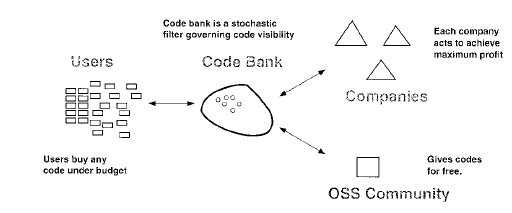
\includegraphics{Figura_1.png}
\section{Variables}
Visibilidad: ${V_{ij}=(i-b_r)[(1-b_p)A_i + b_p M_i] + b_r X_{ij}}$\\
${i}$ - compa\~n\'ia \\
${j}$ - usuario \\
${A_i}$ - publicidad de la compa\~n\'ia \\
${M_i}$ porci\'on del mercado \\



\end{document}  
